\chapter{Сферический трехосный пассивный электростатический подвес} \label{chapt3}

% \section{Определение главного вектора сил и главного момента для сферического тела в электростатическом подвесе} \label{sect3_1}

% \section{Анализ жесткости электростатического подвеса для различной формы электродов}\label{sect3_2}

\section{Краткое описание объекта исследования – трехосного пассивного электростатического подвеса, некоторые аналитические оценки} \label{sect3_1}

Объектом исследования является упрощенная схема трехосного электростатического подвеса, приведенная на рис. \ref{img:sphere_susp_scheme}. Построим конечно-элементную модель в программной системе ANSYS, принимая следующие допущения:
\begin{enumerate}
  \item Центр тяжести сферического ротора совпадает с его геометрическим центром
  \item Каналы X, Y, Z подвеса строго ортогональны друг другу
  \item Результирующая пондеромоторных сил каждого из каналов X, Y, Z в любой момент времени действует вдоль оси своего канала
  \item Результирующий вектор момента сил равен нулю
\end{enumerate}

\begin{figure}[ht]
    {\centering
        \hfill
        \subbottom[List-of-Figures entry][Упрощенная схема трехосного подвеса\label{img:sphere_susp_scheme}]{%
            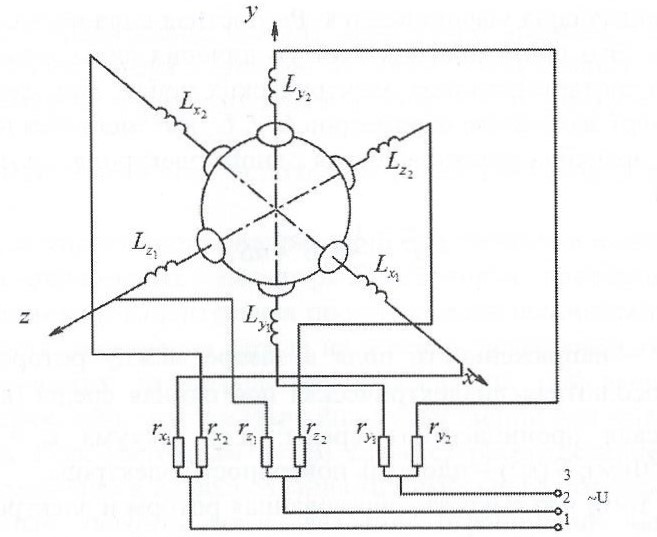
\includegraphics[width=0.49\linewidth]{sphere_susp_scheme}}
        \hfill
        \subbottom[Эквивалентная электрическая схема подвеса\label{img:sphere_susp_el_scheme}]{%
            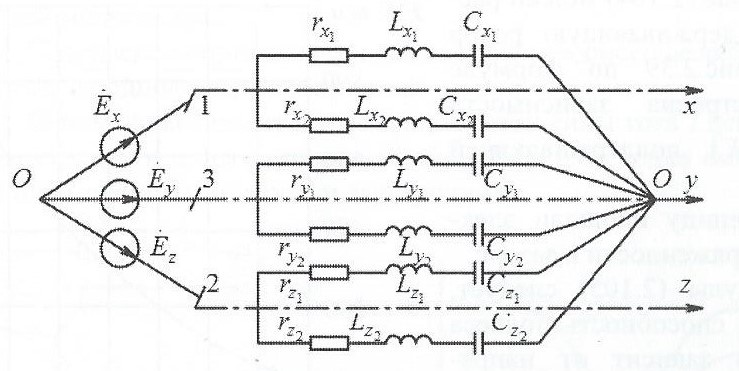
\includegraphics[width=0.49\linewidth]{sphere_susp_el_scheme}}
        \hfill
    }
    \caption{Сферический трехосный пассивный электростатический подвес: схемы}
    \label{img:sphere_susp_schemes}
\end{figure}


С учетом введенных допущений конечно-элементную модель построим следующим образом: электрические цепи моделируем \textit{CIRCU124} элементами, сферический ротор представим точечным элементом массы \textit{MASS21}, емкости, образованные ротором и фиксированными обкладками каждого из каналов, моделируем электромеханическими элементами-преобразователями \textit{TRANS126}.

Для задания в электромеханических элементах \textit{TRANS126} зависимости электрической емкости от величины зазора $C(\delta)$ построим вспомогательную модель и произведем расчет емкости с помощью макроса \textit{CMATRIX}. Вспомогательная модель представляет собой полость между фиксированными электродами цепи и ротором, заполненную электростатическими \textit{SOLID122} элементами. Как и в предыдущей главе, итерационно находим зависимость электрической емкости от величины зазора $C(\delta)$ и передаем значения в определение электромеханических элементов.

Динамика подвеса в специализированной литературе \cite{Electropribor} оценивается следующими приближенными уравнениями движения:

\begin{equation}
  \label{eq:sphere_susp_motion}
    \begin{alignedat}{2}
    &L \frac{d^2 \Delta i}{dt^2} + R \frac{d \Delta i}{dt} + \frac{1}{C_0} \Delta i = B \Delta \dot x \cos{(\omega t - \phi)} - B \omega \Delta x \sin{(\omega t - \phi)}, \\
    &m \Delta \ddot x + F_x = mg.
    \end{alignedat}
\end{equation}


\noindent где $B = \frac{u_0}{ \delta_0 C_0 \omega \sqrt{R^2 + (L \omega -1/C_0 \omega)^2} }$, $\Delta i,\ \Delta x$ – отклонение соответствующих параметров от начальных значений, $i(t) = \frac{dq(t)}{dt}$ – связь тока с зарядом. 

Подбор параметров системы производится таким образом, чтобы величина $\eta = 1$ \cite{Electropribor}:

\[
\eta = \frac{L\omega - \frac{1}{C\omega}}{R} = 1
\]

Тогда параметрами подвеса выберем:
\begin{itemize}
  \item Амплитуда источника напряжения $u_0 = 30\ \text{кВ}$
  \item Частота источника напряжения $\omega = 500\ \text{кГЦ}$
  \item Сопротивление резистора $R = 3636\ \text{Ом}$
  \item Индуктивность $L = 80\ \text{мГн}$
  \item Номинальный зазор $\delta_0 = 40\ \text{мкм}$
  \item Масса удерживаемого твердого тела $m = 1.0\ \text{мкг}$
  \item Площадь фиксированного электрода $S = 3\ \text{см}^2$
\end{itemize}



\section{Результаты конечно-элементного моделирования трехосного пассивного электростатического подвеса}

Динамический анализ производим методом Ньютона-Рафсона, время расчета $30$ мс, шаг интегрирования $dt_{max}=\frac{1}{64} \cdot T,\ T=1/\omega$. Зададим ротору ускорение вдоль оси Z $a_z = g = 9.8 \text{м}/\text{с}^2$, моделируя силу тяжести. Для проверки корректности работы подвеса вдоль всех осей добавим ускорение вдоль оси X, $a_x = 4 \text{м}/\text{с}^2$.

На рис. \ref{img:sphere_susp_u} приведены перемещения ротора по трем осям X,Y и Z. Как и в случае с одноосным подвесом, собственное движение трехосного подвеса неустойчиво и для обеспечения устойчивости необходимо в схему управления вводить коррекционные цепи, обеспечивающие демпфирование механических колебаний ротора. Без демпфирующих слагаемых в подвесе происходит постоянная «накачка» энергии, амплитуда механических колебаний растет до момента столкновения ротора с одним из электродов. 


\begin{figure}[ht] 
  \centering
  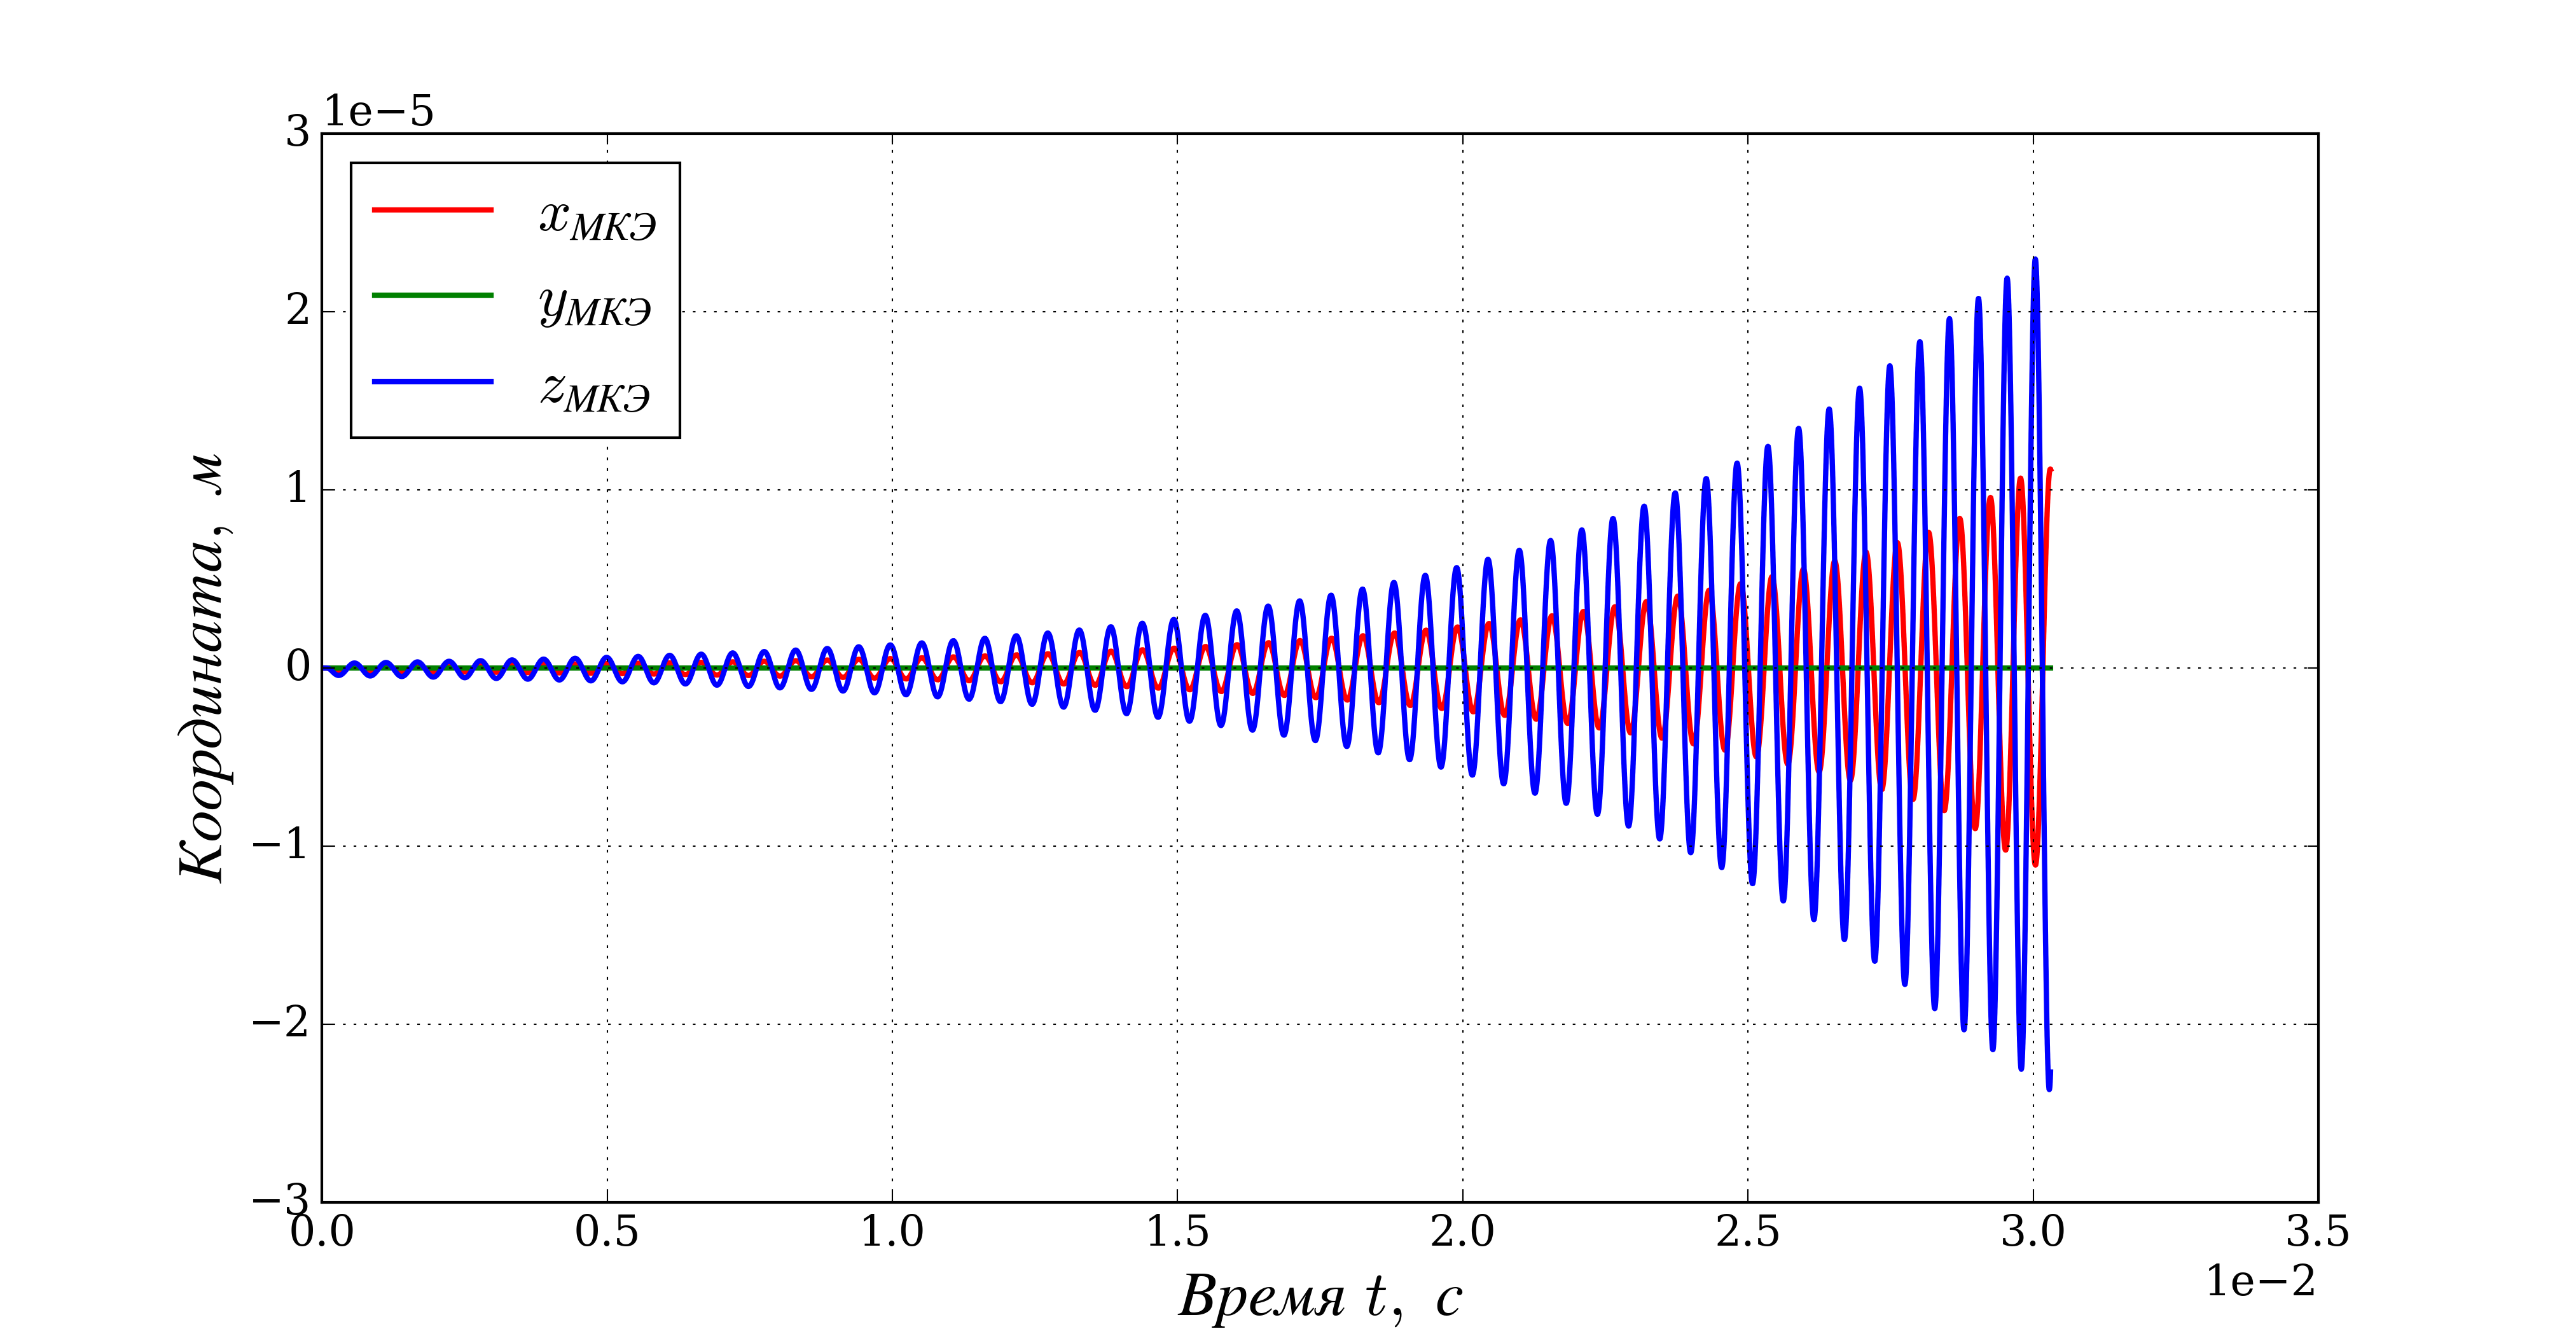
\includegraphics [scale=0.5] {sphere_susp_u}
  \caption{Результат конечно-элементного моделирования: перемещения ротора}
  \label{img:sphere_susp_u}
\end{figure}

Плотной «закраске» на рис. \ref{img:sphere_susp_volt} и \ref{img:sphere_susp_force} соответствуют быстрые колебания заряда с частотой источника $\omega$ и $2\omega$ соответственно.

\begin{figure}[ht] 
  \centering
  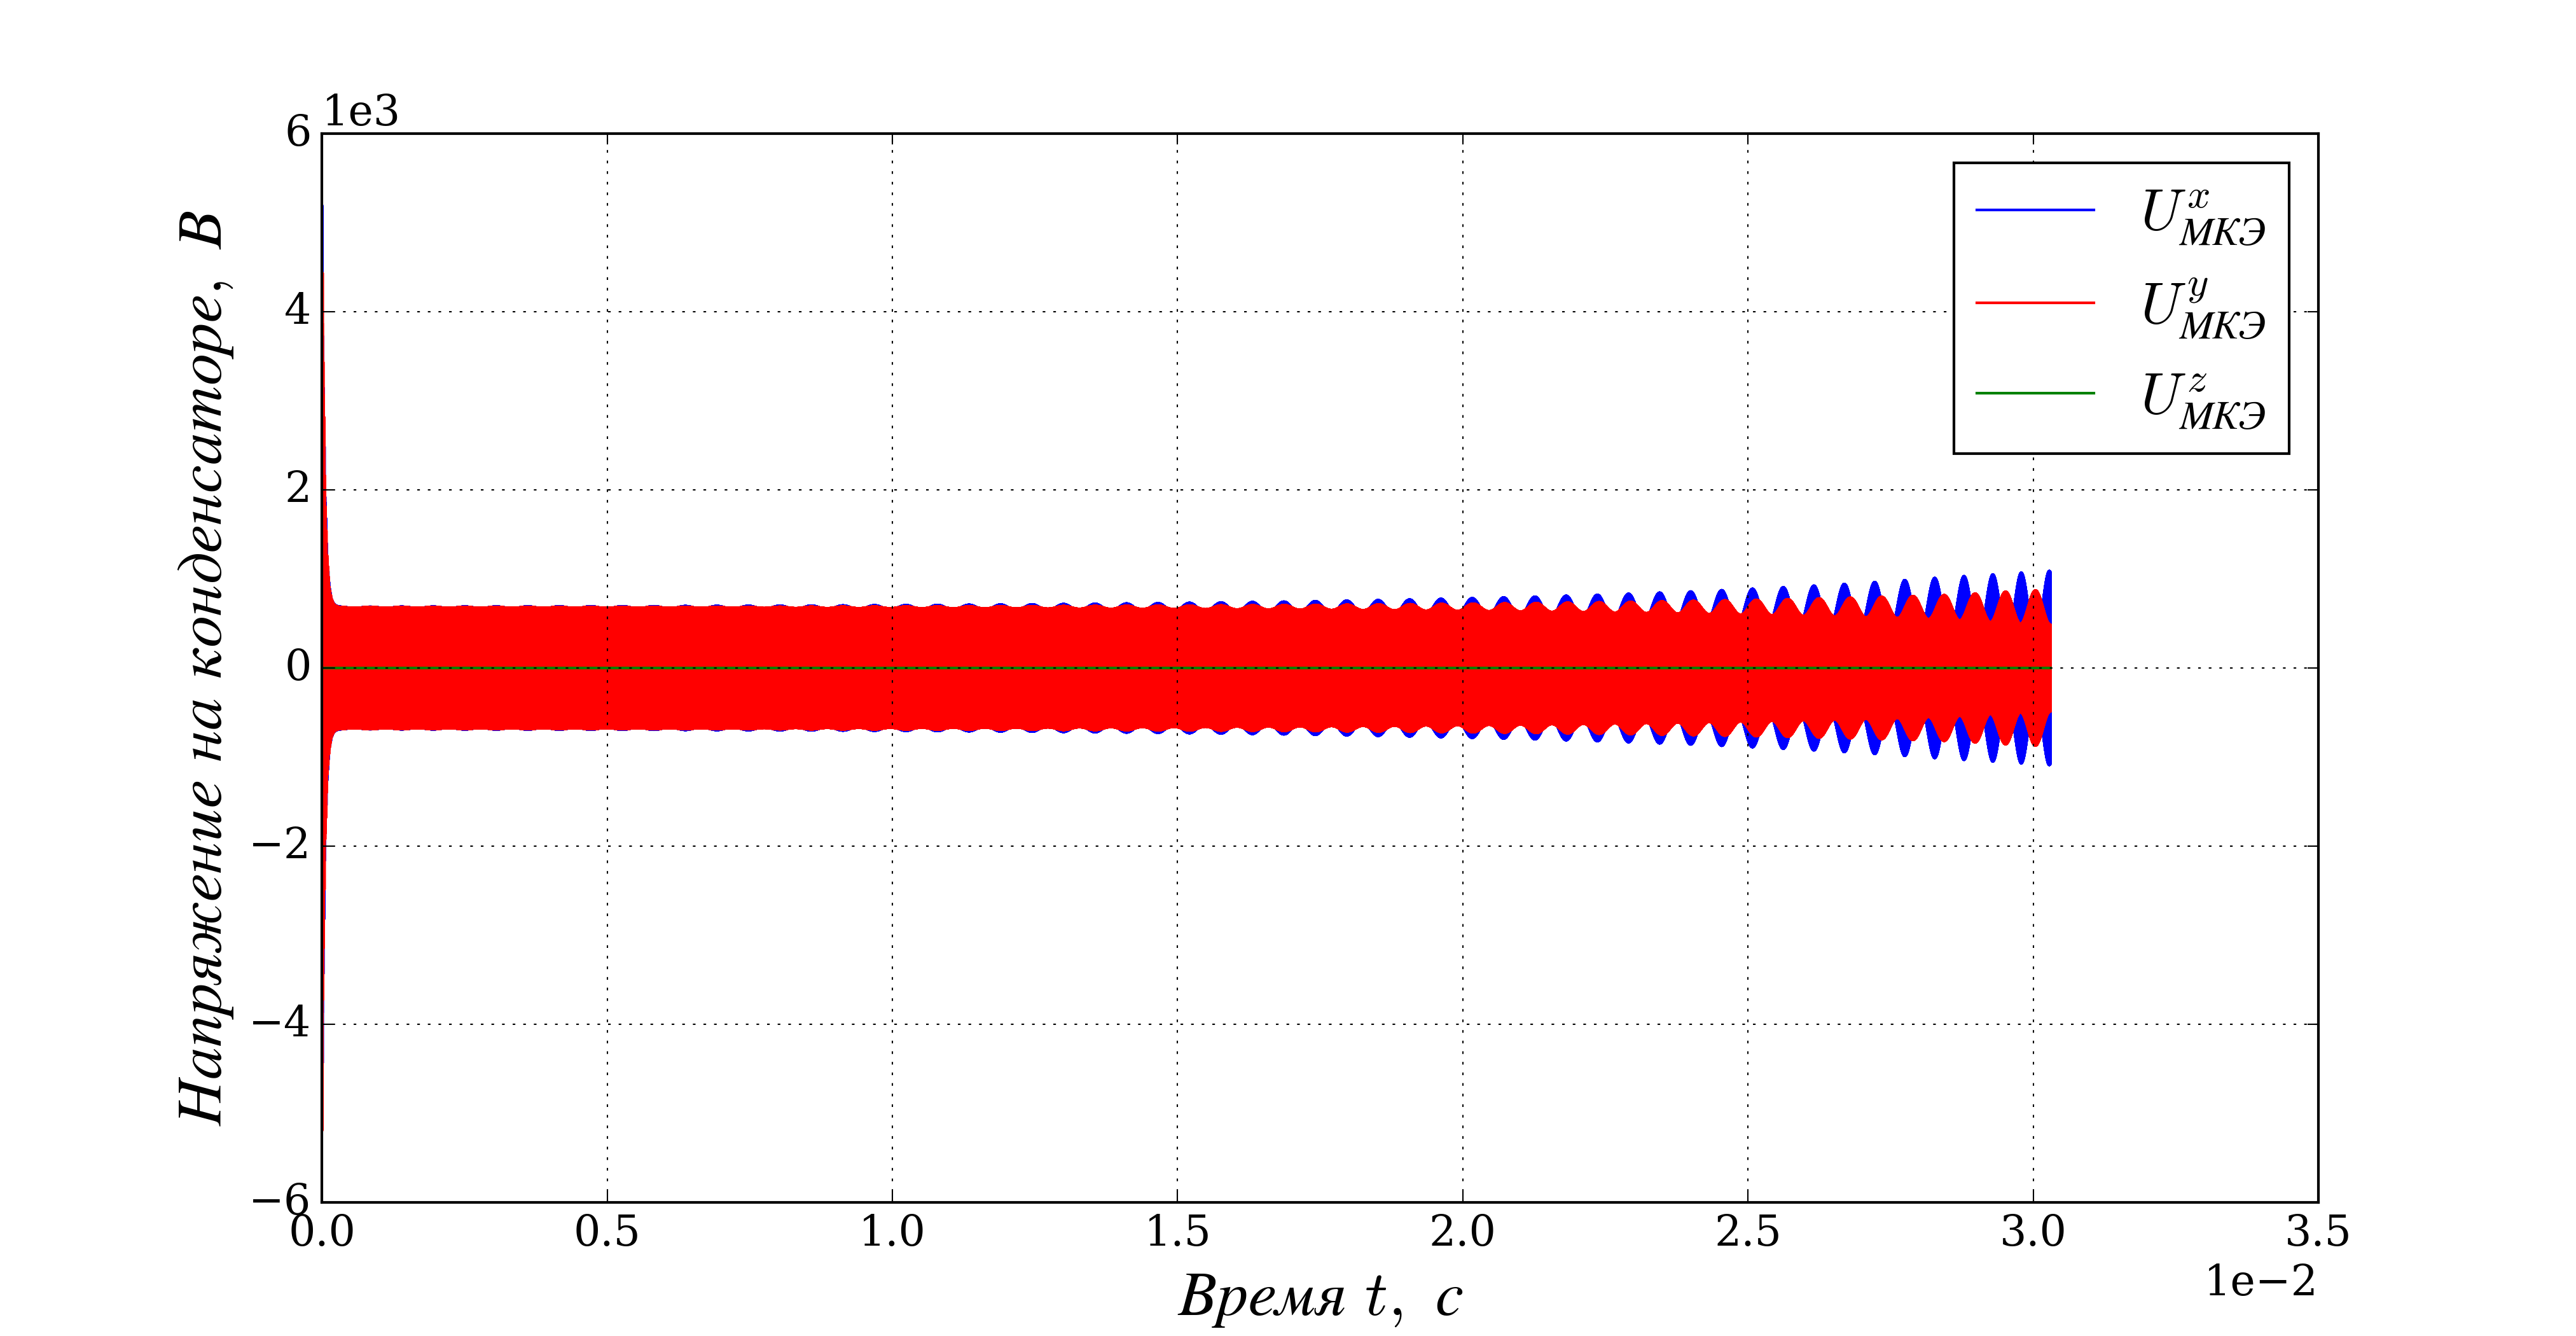
\includegraphics [scale=0.5] {sphere_susp_volt}
  \caption{Результат конечно-элементного моделирования: напряжения на конденсаторах}
  \label{img:sphere_susp_volt}
\end{figure}

На рис. \ref{img:sphere_susp_force} особенно ярко выражено затухание общего решения электрической части уравнения движения цепи или, иначе, затухания переходных процессов электрического контура.

\begin{figure}[ht] 
  \centering
  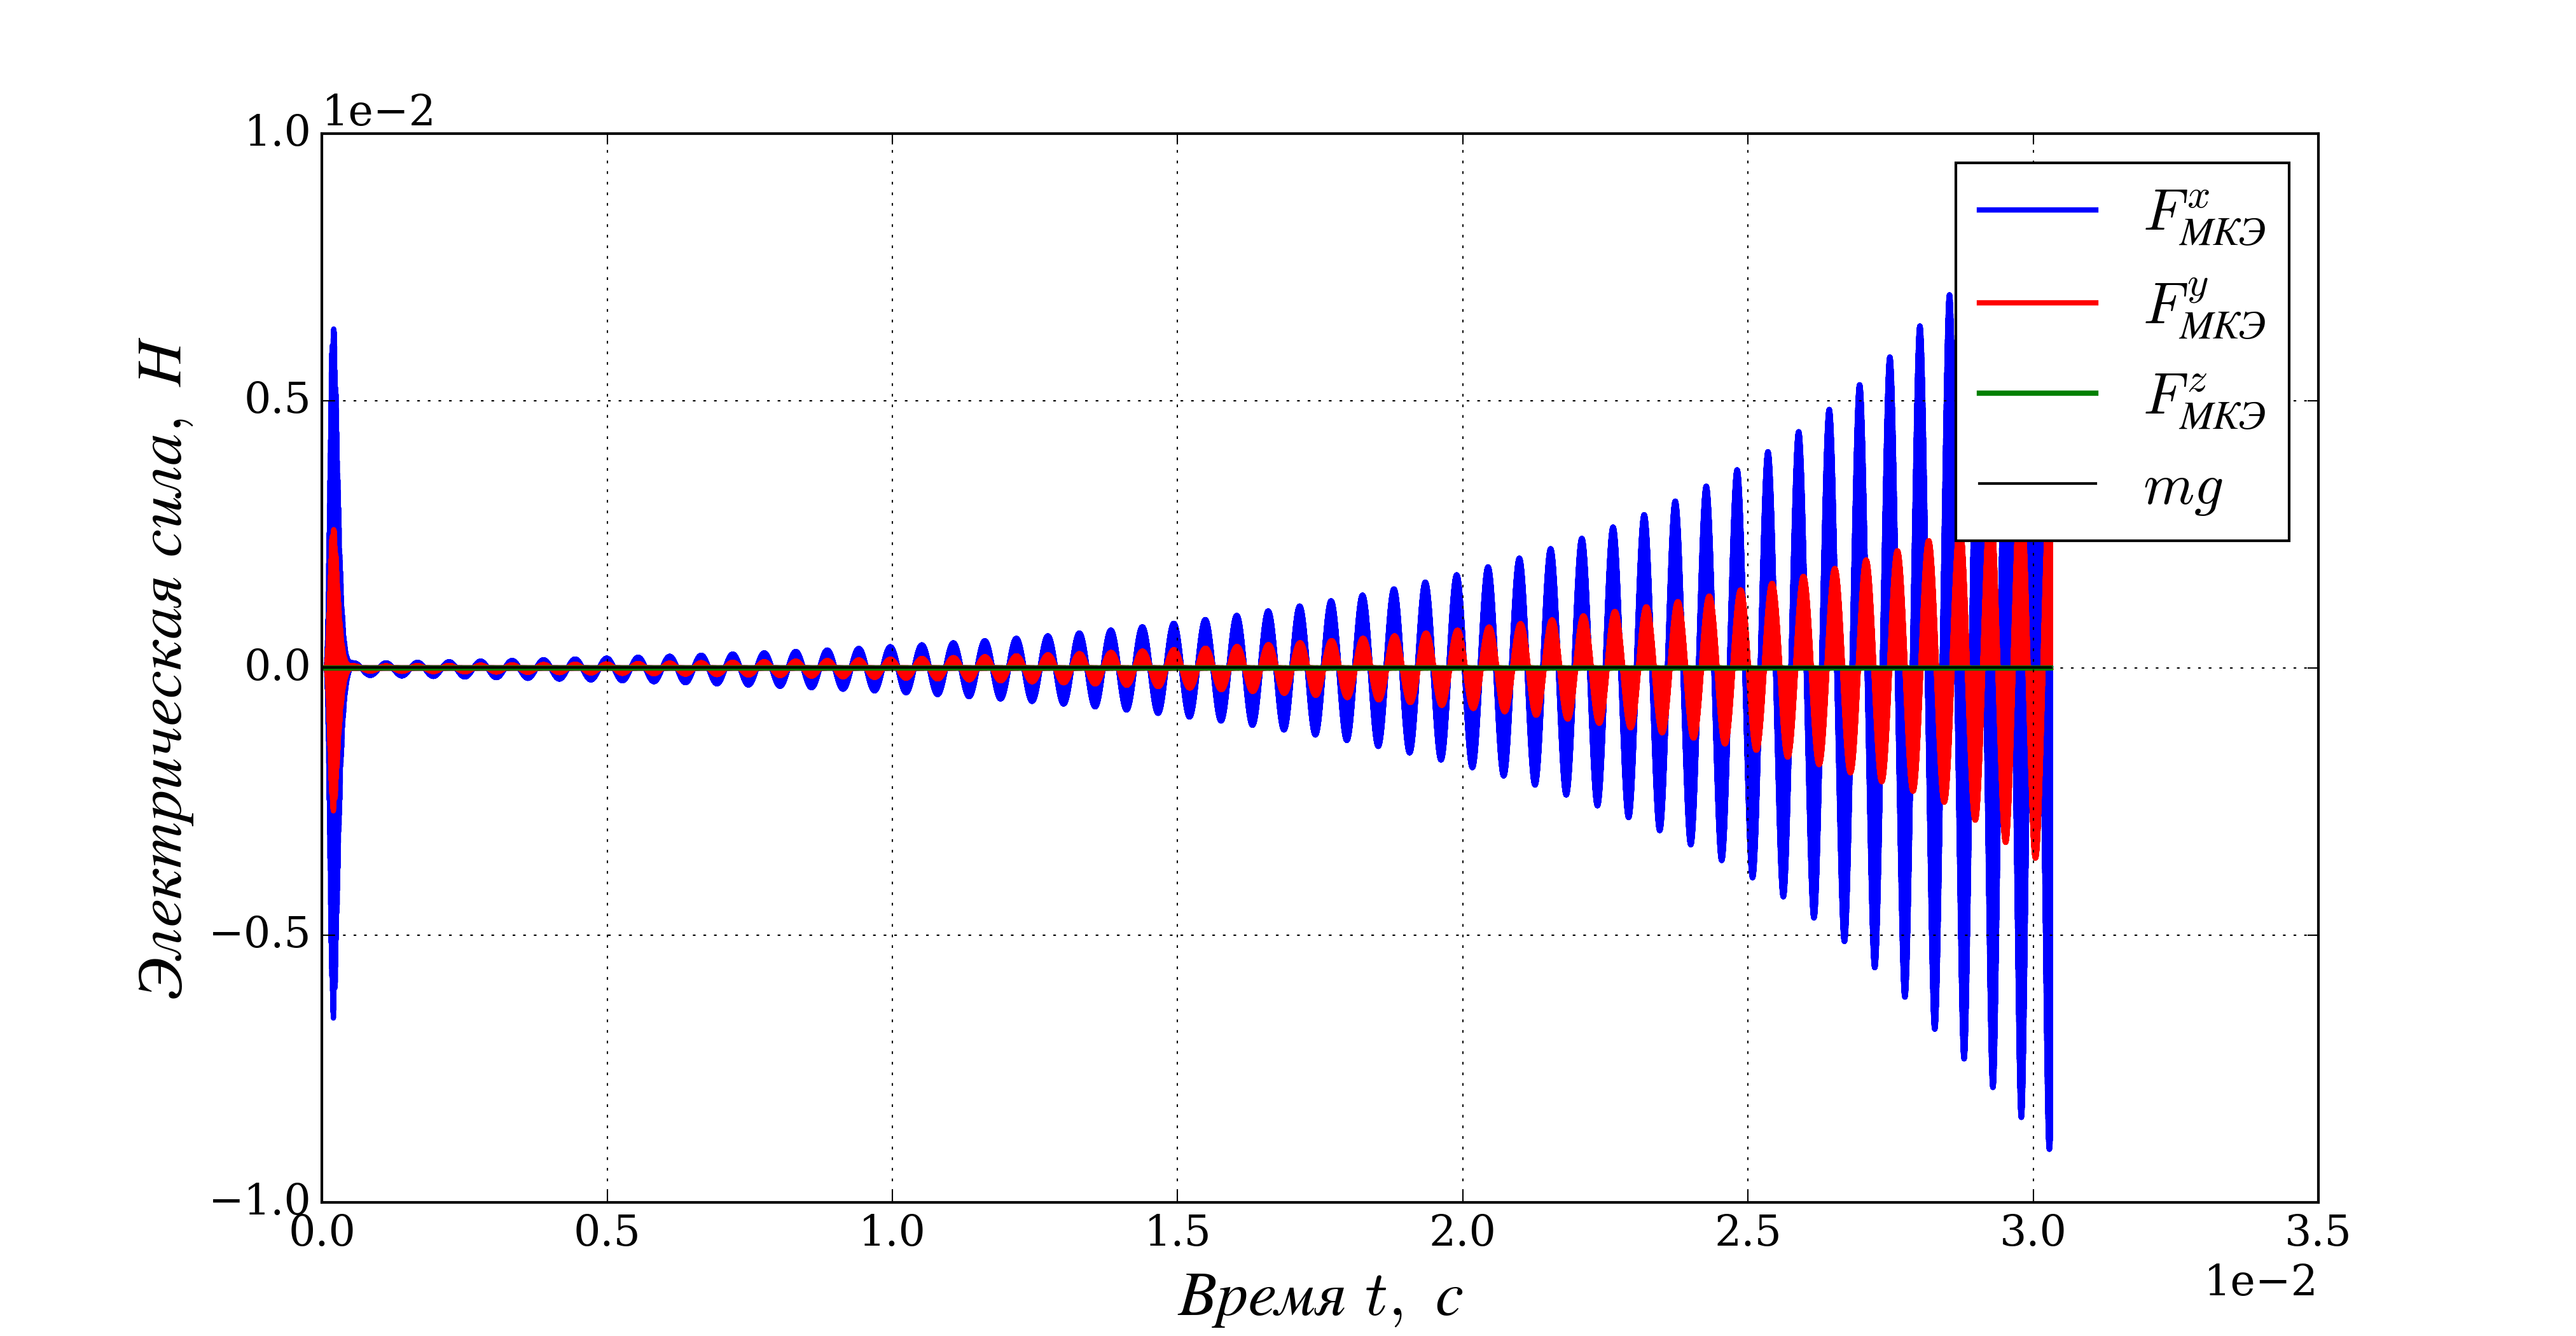
\includegraphics [scale=0.5] {sphere_susp_force}
  \caption{Результат конечно-элементного моделирования: электрические силы}
  \label{img:sphere_susp_force}
\end{figure}

Таким образом, для упрощенной модели трехосного электростатического подвеса получено конечно-элементное решение динамической задачи методом Ньютона-Рафсона. Продемонстрированы возможности программной системы ANSYS для решения трехмерных электромеханических задач. Подготовлена конечно-элементная модель трехосного пассивного подвеса по упрощенной схеме.

% \section{Учет несферичности ротора в конечно-элементной модели}

